%!TEX root = ../username.tex

%%%%%%%%%%%%%%%%%%						
%    Chapter 0   %
%%%%%%%%%%%%%%%%%%
\chapter{Introduction}\label{intro}

%key aspects of a virtual reality: virtual world, immserion, sensory feedback, interactivity



%The key elements that makes a virtual experience immersive To understand and create a solution to this problem requires an understanding the critical factors that make up an immersive experience.

One of the largest roadblocks to virtual reality (VR) is creating a successfully immersive experience for a user. The key elements that bring a virtual reality to life  are a virtual world, immersion, sensory feedback and interactivity \cite{sherman}. This paper focuses on sensory feedback and interactivity, specifically interaction systems within a virtual environment that use haptic feedback technology. This chapter provides a brief history of VR and its applications, immersion is explained followed by an introduction of human perception (touch, sight and sound). After an introduction to VR and the role touch, sight and sound play in creating virtual presence, two interaction systems are described that are used with haptic controllers in Unity to create immersion through object interaction. A VR application is created to demonstrate the effect a Newtonian object interaction system has in a virtual environment and its effectiveness in promoting an immersive experience for the user. The goal of this project is to collect the theory regarding human biological and cognitive interaction systems and transfer this knowledge into making a successfully immersive VR application using Unity 5 and the HTC Vive head-mounted display and haptic hardware.


% Since there are countless sub components that work together to create a sense of immersion, this paper will just focus primarily on one of the most important immersive components, interaction systems with a virtual environment using haptic feedback and technology. #oldsentence



\section{Defining Virtual Reality}\label{defining VR}

As a growing field, the definition of virtual reality is still in flux and has grown to mean different things in certain contexts. Users of VR naturally have their own interpretations, which differ based on their levels of familiarity with the field.  Therefore, it is important to keep the reader grounded to one formal definition of VR in the context of this paper that can be used as a frame of reference. A formal definition is as follows:


\begin{quote}
	A medium composed of interactive computer simulations that sense the participant's position and actions, providing synthetic feedback to one or more senses, giving the feeling of being 
	immersed or being present in the simulation \cite{craig}.
\end{quote}

In other words, virtual reality is a place that exists that we can interact with and experience. In order to create a virtual reality, a virtual world is presented that appeals to our senses in a similar way people perceive reality. VR's singular goal is to display an illusion so successful that the user believes they are somewhere else entirely. 


\section{History}\label{History}


Although VR seems like a fairly new science, the concept stretches all the way back to the 1930's. Alders Huxley and Stanley Weinbaum wrote books imagining movies that extend past just sight and sound to include taste, smell and even touch \cite{mihelj_apps}. These sensory additions work to displace the viewer from their current reality and immerse them in another. 


\par The first concepts of VR were brought to life around 20 years later by a man named Morton Heilig. Heilig created a machine called the \textit {Sensorama}, which offered a virtual bicycle riding experience \cite{mihelj_apps}. This machine enabled the user to observe a three-dimensional display while listening to sounds of a city and experiencing the wind, vibrations and even smells that one would perceive on a real bike ride.

\begin{figure}[h]
	\centering
	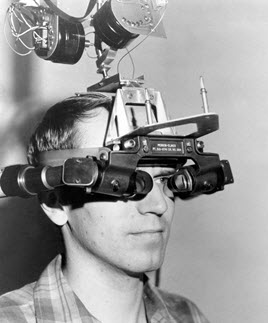
\includegraphics[width=0.4\textwidth]{photo1_sutehrland}
	\caption{Sutherland's Head Mounted Display \cite{photo1_Sutherland}.}
	\label{fig:sutherland_Display}
\end{figure} 


\par In 1976, this innovative technology led Ivan Sutherland to create the first head mounted display that was connected to a virtual environment, seen in figure \ref{fig:sutherland_Display}. Similar to modern virtual hardware, Sutherland's display consisted of glasses with two small screens that created the illusion of three-dimensional vision. The display allows the user to change what they observed by moving their head. This technology required a complex motion tracking system attached to the ceiling. Although groundbreaking, Sutherland's device did not let the user interact with the virtual environment.

\par Even though the technology did not exist, Sutherland had a vision of an ultimate stage of VR development, and how it could be achieved. A challenge was set that has motivated the progress of VR ever since: 

\begin{quote}
	The screen is a window through which ones sees a virtual world. The challenge is to make that world look real, act real, sound real, and feel real  \cite{gobbetti}. 
\end{quote}

The challenge was accepted by a man named Myron Kreuger, who coined the term artificial reality around 1970. Krueger created the first virtual system that allowed a user to interact with objects in a virtual environment. Through various sensors, the user's activities were monitored, allowing feedback within the program. Virtual object interaction was a major advancement towards completing Sutherland's challenge and inspired many new technologies to follow suit.  

Since Kreuger, VR development has continued to grow and become more popular, seeing many new innovations. VR in the media played a huge part in the popularization of the term. Movies like Tron and the Matrix imagined virtual worlds so advanced that distinguishing them from reality became nearly impossible. Though VR technology advancements continued through the 70's and 80's, Sutherland's challenge had only been achieved through film and imagination. 
In the 1990's, the Cave Automatic Virtual Environment, or CAVE was created.

\begin{figure}[h]
	\centering
	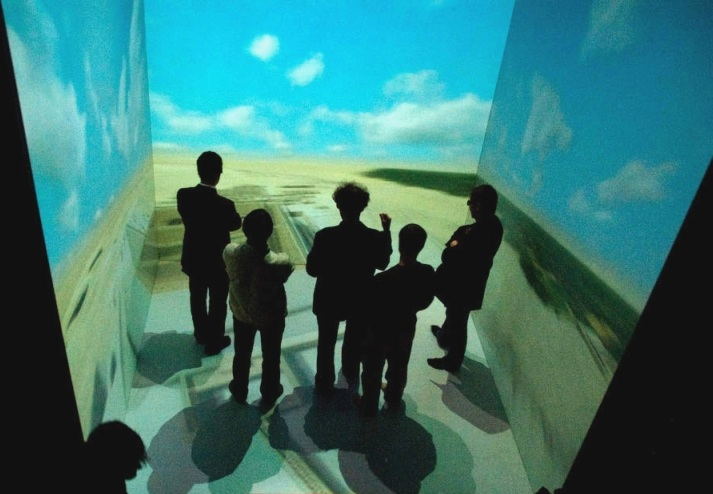
\includegraphics[width=.55\textwidth]{photo16_cave}
	\caption{CAVE: 4 Screens With 4 Stereoscopic Projectors \cite{CAVE}.}
	\label{fig:cave}
\end{figure}


CAVE was a large room full of screens that displayed a virtual environment, taking a different approach to VR hardware \cite{mihelj_apps}. One could also wear special glasses that made objects seem more three-dimensional in the eyes of the user. In addition, special sensors and surround sound were also used to promote immersion. Something else unique about this hardware was that and multiple users could fit in a Cave, enabling collaboration within the virtual environment. In just 60 years, the concept of VR was born and turned into a reality. Today, perfectly immersive virtual worlds have yet to be achieved, but the advancements and uses of VR have reached heights previously thought impossible. 



\section{Applications}\label{Apps}

Virtual Reality enables people's imaginations to run wild. Although the age of consumer VR is just beginning, the current range of applications is tremendous. One of the most prevalent areas of VR is within the gaming industry. Virtual reality gives gaming the potential for a user to become immersed in the virtual world. In lieu of a keyboard and mouse, haptic hardware gives users the opportunity to interact with virtual objects on a whole different level, changing immersive gaming as we know it. The potential for deep immersion, virtual presence and the production value  VR has to offer as an industry is driving developers and manufacturers to take part in the emerging field \cite{parisi}.   

 \begin{figure}[h]
	\centering
	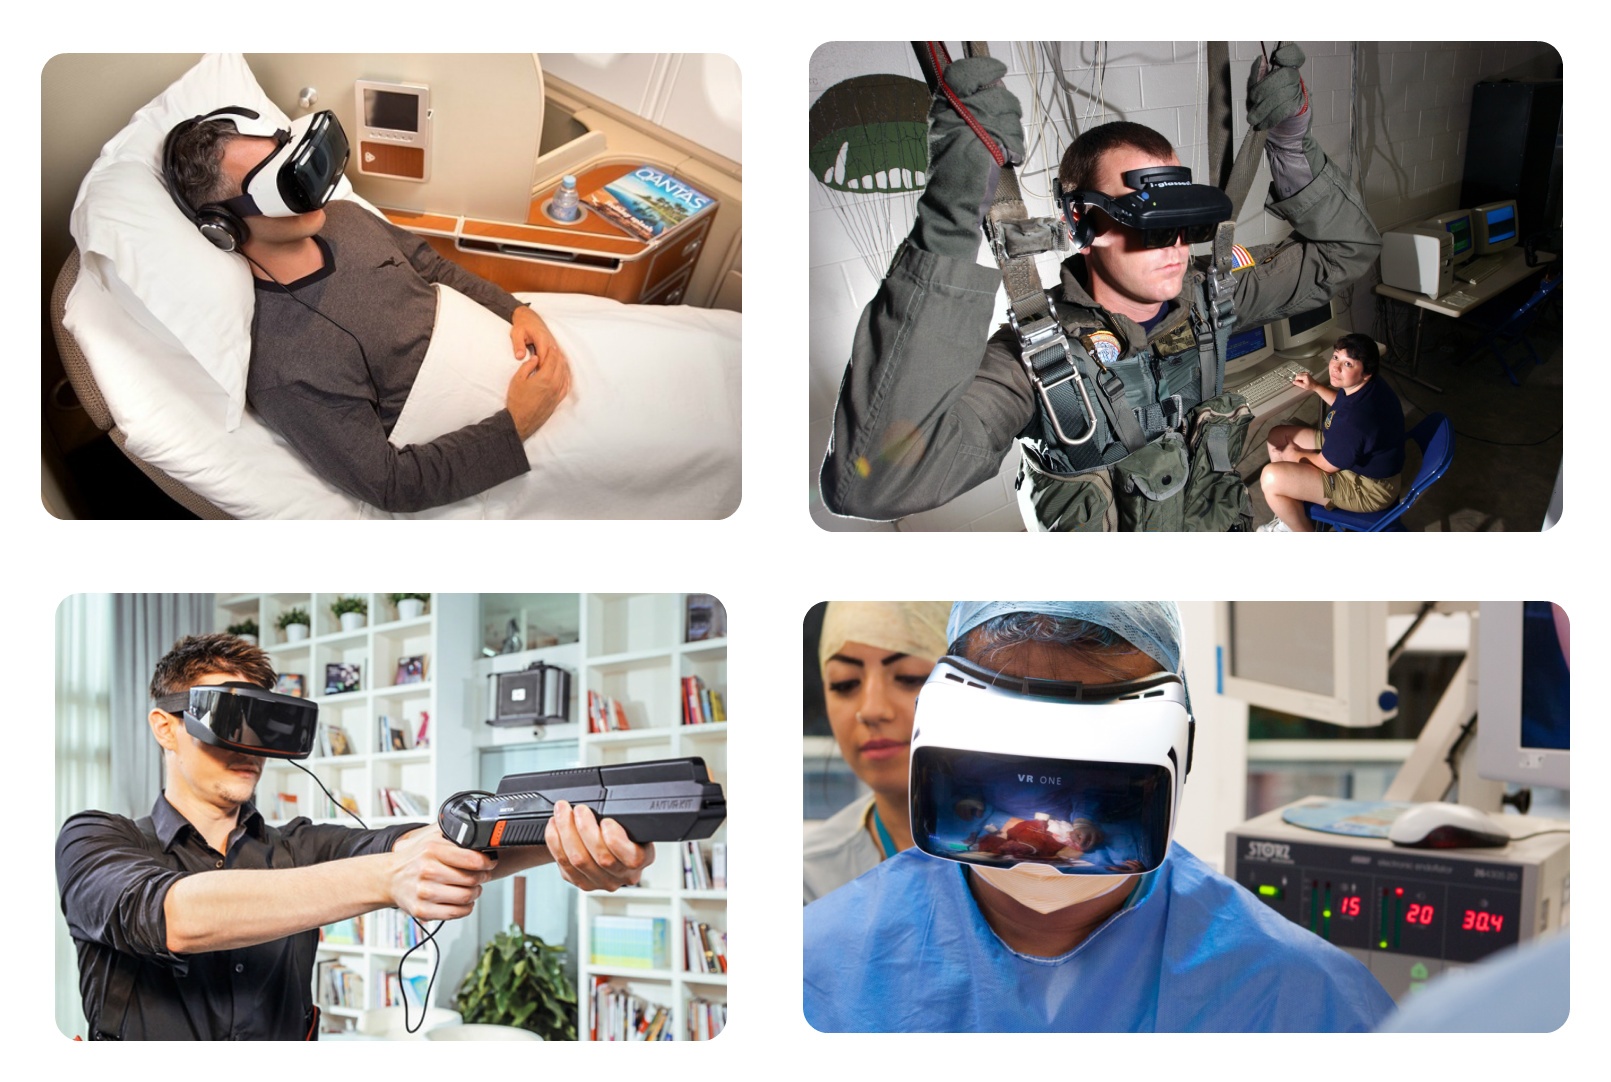
\includegraphics[width=.6\textwidth]{photo8_applications}
	\caption{VR Medical Applications \cite{applications}.}
	\label{fig:applications}
\end{figure}

However, new haptic and visual technology are not just being used for entertainment. Virtual reality is already successfully being used in many other applications, some of which are seen in Figure \ref{fig:applications}. The creation of immersive 3D virtual environments has enabled VR to be used in military training, medical training, and all types of design and engineering.These examples are just the beginning. The potential for VR in our modern day society is endless, ranging from interactive tourism to psychotherapy. With more and more foreseeable applications in todays society, the demand and technological innovations will just continue to increase, making VR development even more prevalent and expansive. 

\section{Virtual Presence}\label{presence}

VR is a unique form of media quite unlike other medias such as books or movies and should be dealt with as such. To acquire virtual presence while reading a book, the reader must leave their current reality behind to enter the reality of the text \cite{mihelj_apps}. VR requires the opposite. With VR, the user is placed into an environment and is meant to perceive and respond to it as though it were real. Virtual presence is the feeling of actually existing within a a virtual environment. In the words of Albert Einstein, reality is merely an illusion, albeit a very persistent one. Creating a successful virtual environment requires the creation of a successful illusion.  An effective illusion is made possible through a strong virtual presence. Virtual presence is achieved mentally, physically, or by a combination of the two. 

\subsection{Physical Presence}\label{physical presence}

Physical presence is an essential part of VR and takes place when the user's body physically enters the simulation or environment. It is truly what sets VR apart from other media.  In response to the users actions, select stimuli are presented to the user that affect their perception of the environment. Specifically, virtual environments are described through sight, sound and touch. These sensory perceptions define user interaction in a virtual world and are described in greater detail in the following section. 
	
\par The goal to obtaining optimal virtual presence is reducing as much real world stimuli as possible.
When immersed in the environment, virtual stimuli work to replace the user's exposure to real stimuli, decreasing mental and physical presence in the real world. Physical and mental presence go hand in hand. If physical stimuli are tricked to make you think you are present in a different environment, your mental presence in that environment also increases. 
	
	
	\begin{figure}[h]
		\centering
		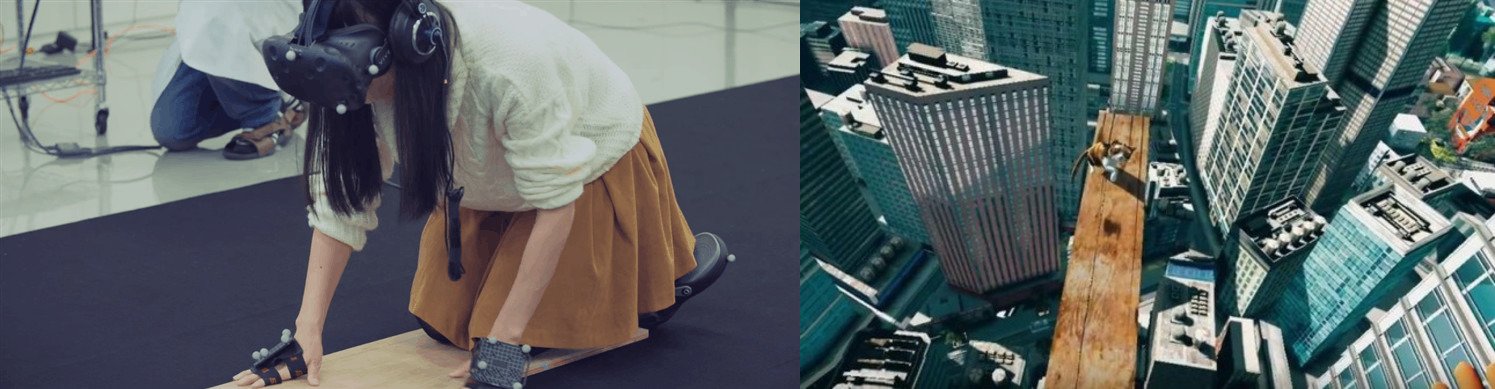
\includegraphics[width=\textwidth]{savecat}
		\caption{Virtual Presence: Fear of heights - save the cat or die trying \cite{matulef}.}

		\label{fig:savecat}
	\end{figure}
	
	
\subsection{Mental Presence}\label{mental presence}
	
	
It is possible for a user to be so immersed in a virtual world that it becomes their reality. Figure \ref{fig:savecat} is an example of a game made by Bandai Namco that challenges the user to save a cat from a wooden plank suspended thousands of feet in the air. This game creates mental presence by provoking very real fear among its users, so real that many are not able to save the cat successfully. Mental presence is the non-physical state of engagement felt after entering a virtual world. Achieving and maintaining mental presence is a very delicate and complicated process. There are many factors that affect mental presence. This also means many factors can destroy an immersive process. For example, a sense of virtual realism can be destroyed by small environmental defects because they distract the user from perceiving the scene as legitimate. The level of mental  presence is affected by the virtual scenario, the quality of realism, the number of senses stimulated, and the delay between the users actions and its effect on the virtual world. Mental presence within a virtual reality is difficult to achieve because all of these factors must be taken into account. In order to  successfully obtain virtual presence, a minimum level of physical and mental presence is key.  

\section{Conclusion}\label{intro_conclusion}

Virtual reality has a rich history and a bright future. The technological advances VR has made in the past 60 years and the current range of applications show the incredible potential of the growing field. For a virtual environment to be immersive, both the mind and body must believe they left their world behind and entered a new one. Physical and mental presence are crucial for a virtual space to be successful. The next chapter dives into the human sensory system and why it must be understood in order to model immersive environments that successfully capture the physical and mental presence of a user. 

